\begin{singlespacing}
\chapter{Data analysis and \atlas\ searches}
\label{chapter:searches}
\begin{epigraphs}
\qitem{%
One way is to make it so simple that there are \emph{obviously} no deficiencies
and the\\
other way is to make it so complicated that there are no \emph{obvious}
deficiencies.%
}%
{Tony~Hoare,
\textit{The Emperor’s Old Clothes},
1981~\cite{hoare2007emperor}}
\end{epigraphs}
\end{singlespacing}
\noindent
Our aim in scientific data analysis is to distil useful messages from the
data, and to report that message to the wider community.
Various messages could be extracted from any given data,
and those messages will have varied values to their recipients.
Data analysis is not an automatic process, but a design with many judgements
that are informed by theory, intuition, and convention to give value to their
results.

To support our later description of the \atlas\ SUSY `$\twoljets$' search in
Chapter~\ref{chapter:2ljets}, this chapter introduces the basic theory of
data analysis and its conventional form in the \atlas\ SUSY
community, parts of which can only be explained in their historical context.

Theoretical data analysis in the tightly coupled fields of probability theory
and decision theory is introduced in Section~\ref{sec:searches_data_analysis}.
An attempted alternative formulation, frequentist theory, is discussed in
Section~\ref{sec:searches_frequentist} for its relevance to our methods.
Standard practice in this field of research does not strictly follow
frequentist methods, but patches up some of their pathologies with modified
approaches that we describe in Section~\ref{sec:searches_practice}.
Searches for supersymmetric signals in \atlas\ follow a standard strategy for
their data analysis, whose procedures, nomenclature, and parametric modelling
are introduced in Section~\ref{sec:searches_searches}.


\section{Data analysis}
\label{sec:searches_data_analysis}
How many jelly beans are in the jar of Figure~\ref{fig:searches_beans}?
Your guess depends not only on what you observe from the figure, but also on
what else you know about cartoon jars of beans, and on what reward is offered.
Each answer is a decision, which depends both on how you value the rewards,
and on which numbers of beans you subjectively infer to be probable.
We return to this example after developing its analysis in probability
and decision theory.

\begin{figure}[tp]
\centering
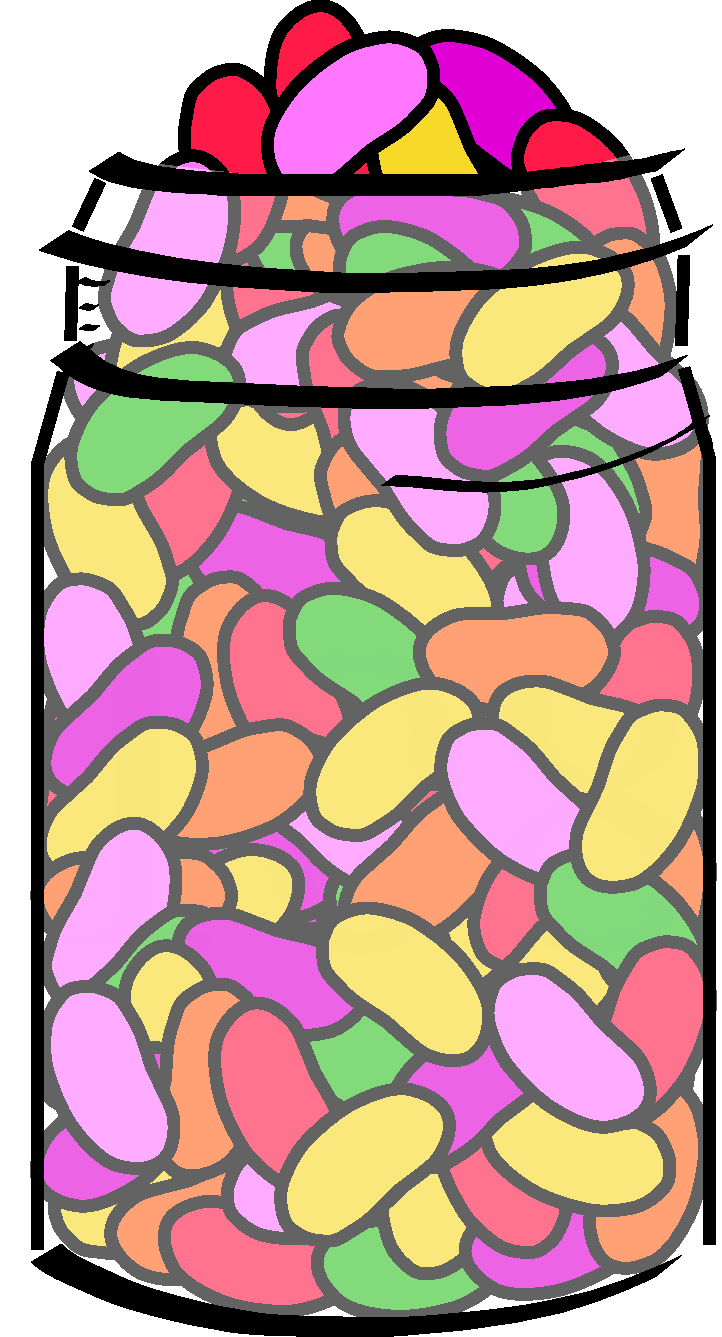
\includegraphics[width=0.25\textwidth]{figures/searches_beans.pdf}
\caption[
How many beans are in the jar?
]{%
How many beans are in the jar? This jar of jelly beans is a vehicle for our
discussion of inference and decision theory.
Please write your guess on this page.
The first correct answer wins a gold star.
}
\label{fig:searches_beans}
\end{figure}

Statistical data analysis suffers from dogma --- prescriptions and recipes that
one memorizes and follows without necessarily knowing their reasons or their
limitations:
among these are
error propagation formulae,
least-squares fitting routines,
chi-squared per degree of freedom,
and myriad statistical tests with \pvalues\ and confidence intervals.
Each of these can be a useful approximation, but every one can also fail if
misused outside its domain.%
\footnote{%
Multiplicative error propagation is an example:
for independent $a = \mu_a \pm \sigma_a$ and $b = \mu_b \pm \sigma_b$,
the standard rule says
\(
\widetilde{\sigma}_{ab}
= \mu_a \mu_b \sqrt{\sigma_a^2/\mu_a^2 + \sigma_b^2/\mu_b^2}
% = \sigma_a^2 \mu_b^2 + \sigma_b^2 \mu_a^2
\),
but a calculation with their moments derives the exact result
\(
\sigma_{ab}
= \sqrt{(\mu_a^2 + \sigma_a^2)(\mu_b^2 + \sigma_b^2) - \mu_a^2\mu_b^2}
% = \sigma_a^2 \mu_b^2 + \sigma_b^2 \mu_a^2 + \sigma_a^2 \sigma_b^2
\);
since $\sigma_{ab}^2 = \widetilde{\sigma}_{ab}^2 + \sigma_a^2 \sigma_b^2$
the propagation formula assumes at least one small relative error.
}
All effective methods of data analysis can be justified in probability and
decision theory.
As throughout physics, knowing a method's derivation allows one to judge when
its approximations should hold and when it leaves room for improvement.

Probabilistic data analysis follows the ordinary structure of science:
write down predictive models, test their predictions against data,
then update your models (or invent new ones) to refine their predictions.
Likelihood functions are particularly important to this process because
they quantify predictions.
But not everything is a likelihood.

We begin with what probability is: at its most abstract, a probability is a
proportion of stuff within a larger whole.
Probabilities are useful because proportions have important applications,
and because they can be manipulated and interrelated with an intuitive linear
algebra.
The remainder of this section uses the omnipresent tool of high-energy
physics --- the histogram --- to introduce the structure of probability and
its technical language.


\subsection{Probability: abstract}
A probability $\prob{b}{a}$ is a number that quantifies the proportion
of $b$ within $a$, and can be expressed as a ratio
\begin{equation}
\label{eqn:searches_prob_ratio}
\prob{b}{a} = \frac{m(b, a)}{m(a)},
\end{equation}
in which $m(x)$ is a measure, and the comma `,' means `and'
(logical `and', or set intersection or any other equivalent
thing)~\cite{axioms1010038}.

For example, $\prob{b}{a}$ could quantify the proportion of tea within
a spoon within a cup --- then $m(a)$ measures the content of the cup, and
$m(b, a)$ measures the amount of tea in the teaspoon that is partially
submerged in the cup.
All probabilities are conditional in this definition;
Alone, no $\probc{b}$ exists unless some conditioning information is implicit
from context.

Logic is an important application of probability.
To apply to logical reasoning, $a$ and $b$ are logical propositions and
$\prob{b}{a}$ quantifies the degree to which $a$ implies $b$, with the
limiting cases that $\prob{b}{a} = 1$ when $a$ implies $b$,
and $\prob{b}{a} = 0$ when $a$ contradicts $b$.
Indeed Cox's theorem shows that probability algebra is uniquely consistent
with Boolean logic~\cite{
cox1946probability,
cox1961algebra,
garrett1998nand,
jaynes2003probability,
keynes1920treatise
}.
Probability works for logic, and it works \emph{for tea, too}.

Probability \emph{distributions} $\prob{b}{a}$ spread unit probability mass
across states $b$.
They need not be random distributions of fluctuating $b$s~\cite{
jaynes2003probability,
frankfurt2005on
},
although random processes are a useful application.

Probability algebra derives from
Equation~\ref{eqn:searches_prob_ratio}; it has a \textbf{product rule}
\begin{align}
\prob{c, b}{a} &= \prob{c}{b, a}\times \prob{b}{a},
\label{eqn:searches_product_rule}
\intertext{%
for nested proportions
(a spoon in a teacup in a sink),
and a \textbf{sum rule}%
}
\prob{c\;\textrm{or}\;b}{a} &= \prob{c}{a} + \prob{b}{a} - \prob{c, b}{a},
\label{eqn:searches_sum_rule}
\end{align}
for combinations in a union, with sums over exhaustive sets of outcomes
necessarily normalized to unity.

\subsection{Probability: applied}
\label{sec:searches_probability_applied}
Science involves making predictions, testing those predictions against data,
and reporting what is learned from the results.
Various probabilities are involved in this prediction and learning, and those
probabilities have conventional names that communicate our intended use for
them.
Most important for prediction is a \textbf{likelihood}
\begin{align}
\label{eqn:searches_likelihood}
L(a) &= \prob{b}{a}
\intertext{%
which explores the probabilities assigned to a fixed result $b$
(usually data) from different contexts $a$ (hypotheses).
A likelihood is clearly a probability, but it is not a probability distribution
--- only the left hand argument $b$ forms a normalized distribution.
Alternatively, fixing the context gives a \textbf{prior}%
}
\pi(b) &= \prob{b}{a}
\label{eqn:searches_prior}
\end{align}
normalized probability distribution over results $b$ for a fixed context $a$.

\begin{figure}[tp]
\centering
\begin{subfigure}{\textwidth}
\centering
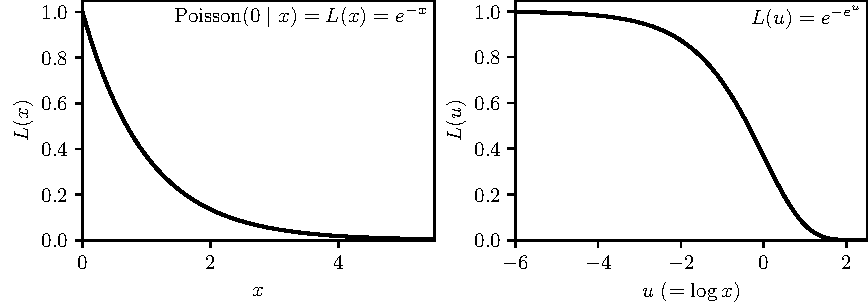
\includegraphics[width=\textwidth]{figures/searches_abacus_likelihood.pdf}
\caption{%
Likelihood: $\mathrm{Poisson}(0\mid x)$ in
(left) $x$ and
(right) $u = \log x$%
}
\end{subfigure}
\\[.5em]
\begin{subfigure}{\textwidth}
\centering
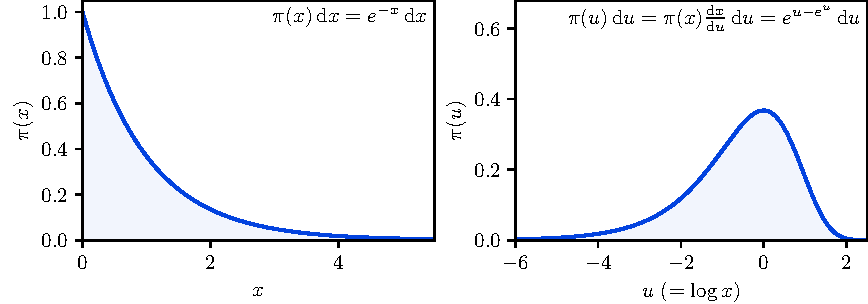
\includegraphics[width=\textwidth]{figures/searches_abacus_prior.pdf}
\caption{%
Prior: exponential density in
(left) $x$ and
(right) $u = \log x$%
}
\end{subfigure}
\caption[
Likelihoods and prior densities' transformations with coordinates.
]{%
Likelihoods and prior densities' transformations with coordinates.
The $\mathrm{Poisson}(0\mid x)$ likelihood and exponential $e^{-x}\mathrm{d}x$
prior have the same form (left).
While the prior density changes to preserve its unit area relative to
$u = \log x$,
the likelihood slides horizontally (right).
Both likelihood maxima are equivalent, but the maximum prior densities change.
}
\label{fig:searches_abacus}
\end{figure}

Since prior probabilities are normalized distributions, it is usually
convenient to represent them as density functions.
Densities are stated relative to coordinates (or measures),
so changing coordinates changes their values as their unit probability mass
is sloshed around.
Likelihoods are not densities,
so changing coordinates instead slides them horizontally like beads on an
abacus, and does not change their values for equivalent states.
Figure~\ref{fig:searches_abacus} illustrates this difference.

Likelihood and prior are evidently related; they explore two indices into
the same object --- two sides of the same coin --- and they are both assigned
by the same principles.
But they are profoundly different objects, which are applied for different
purposes ---
clarity in their distinction will help in our later understanding of
practical methods.
Likelihoods are useful to compare which hypotheses predicted observed data
better than others.
Priors on hypotheses express uncertain predictions, and
priors on data are useful in experimental design.

To illustrate this, we consider a histogram that bins event yields in
$\met$, with distributions from background and (supersymmetric) signal samples
overlaid.
Example such histograms are displayed in
Figure~\ref{fig:searches_sig_bkg_prior_likelihood}.
Since these histograms are normalized to unit area, they show prior
probability distributions along the bin axis.
There is one prior for events from each of the background and signal
hypotheses ---
priors distribute unit probability explore along the bin axis.
In each bin, however, a likelihood function compares the assignments from
the two hypotheses: signal and background ---
likelihoods explore vertically down the sample axis.

\begin{figure}[tp]
\centering
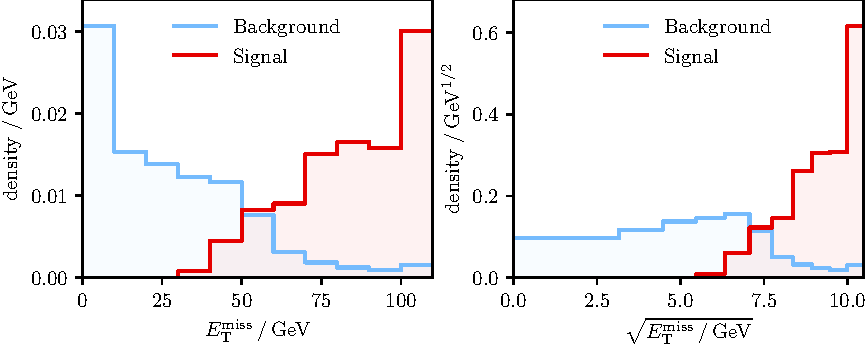
\includegraphics[width=\textwidth]{figures/searches_sig_bkg_prior_likelihood.pdf}
\caption[
Background and signal prior densities
]{%
Background and signal prior densities in $\eV[G]$ and $\eV[G]^{1/2}$ units.
When changing coordinates, probability mass moves as a fluid of constant total
volume, changing its shape in this density view to keep the area of the
rectangle in each bin constant.
A likelihood function indexes each bin in the background--signal labels,
and is independent of the coordinates units, since the area in each bin is
invariant.
}
\label{fig:searches_sig_bkg_prior_likelihood}
\end{figure}

Both distributions are equivalently drawn in two different coordinates
on the left and right of Figure~\ref{fig:searches_sig_bkg_prior_likelihood};
they are identical in content, but differ in appearance because they represent
each prior distribution as a density in the standard way.%
\footnote{%
Density is a somewhat misleading term here ---
probability mass is incompressible; it moves and redistributes more like
depth of water than density of air.%
}
To preserve the area of each bin, which shows its probability mass,
bin heights change to adapt to their width in each coordinate.
Coordinate-dependence of the prior density means that its point of
maximum density is not always meaningful.
But since the probability mass in each bin is constant, the likelihood is
coordinate-independent.

Standard methods approximate such histograms from Monte Carlo simulations.
Simulations do not directly indicate bin indices, but state the values for
event variables;
to connect event variables to bin indices, we begin with some notation:
we have an hypothesis label $h$ (signal or background),
an event variable $x$ that we histogram ($x = \met$),
and we observe a datum $d$ that indexes the histogram bins.
Supposing, for example, that an event is observed in the overflow bin, it says
$d = `x > 100\,\eV[G]\textrm{'}$.
This observed bin has a likelihood function
\begin{equation}
L(x) = \prob{d}{x, h} = \prob{d}{x} =
\left\{
\begin{matrix}
1 & \textrm{if }~x > 100\,\eV[G], \\
0 & \textrm{otherwise} \\
\end{matrix}
\right.
,
\end{equation}
which corresponds to Equation~\ref{eqn:searches_likelihood} by
$b \leftarrow d$ and $a \leftarrow `x, h\textrm{'}$,
and simplifies by $\prob{d}{x, h} = \prob{d}{x}$ because at given $x$ the
binning is independent of any origin from signal or background.%
\footnote{%
Independence of the likelihood function from prior hypotheses is so common
that it should usually be assumed unless otherwise stated.
}
This example of a binary selection highlights how the likelihood acts as a
filter that only rejects events that are contradicted by the data.
Other likelihoods that are not binary act as inefficient filters
that reject events with some probability.

Simulating events from background and signal hypotheses samples from their
respective priors $\pi(x) = \prob{x}{h}$, which
correspond to Equation~\ref{eqn:searches_prior} by
$b \leftarrow x$ and $a \leftarrow h$.
Although we previously used the same labels $a$ and $b$, those are only
labels --- the words `prior' and `likelihood' state our intent to index into
the left and right arguments, respectively.

When we fill a histogram by summing weights of simulated samples, we are
calculating another likelihood over hypotheses $h$ alone in the bin,
which is independent of $x$, by averaging the likelihood over the prior.
This abstracted, $x$-independent likelihood is labelled the \textbf{evidence}:
\begin{align}
Z
= \prob{d}{h} &= \sum_i L(x_i) \,\pi(x_i)
\label{eqn:searches_evidence_integral_sum}
\\
&= \int\! L(x) \,\mathrm{d}\pi(x),
\label{eqn:searches_evidence_integral_measure}
\end{align}
where Equation~\ref{eqn:searches_evidence_integral_measure} is notation for
integrating the likelihood function over the prior measure~\cite{
billingsley2008probability,
skilling2010foundations
},
can be imagined as simulating from the model $\mathrm{d}\pi$ and
counting events that hit pass the likelihood filter.
The name `evidence' relates to its application for model
comparison~\cite{
mackay2003information,
skilling2004nested,
skilling2006nested
}.

Suppose that we have one event with $\met > 100\,\eV[G]$.
Did it come from the background or signal?%
\footnote{%
Questioning the origin of individual events is unusual in our context in
\atlas, but is done in other research into rare effects such as neutrino
interactions and black hole mergers~\cite{
opera2010event,
icecube2020event,
Abbott2021event
}.%
}
The answer depends on the signal and background cross-sections in our collider,
but larger evidence for signal does influence any conclusion to move in its
favour.

Expressing the evidence $Z$ as an average over the prior highlights how it
depends both on how large that likelihood gets,
and on what fraction of samples hit large likelihood values.
Maximum likelihood approaches,
which compare models by the largest likelihoods their priors support,
can be practical and give useful upper bounds on the evidence.
This histogram example, however, highlights a limitation since both models
support the same maximum likelihood of
$L(101\,\eV[G]) = 1$.
These evidence values differ only by their prior masses in the bin.

% posterior
Perhaps we now wanted to see where in the overflow bin this event landed, and
compare the signal and background distributions there.
That would be inspection of the \textbf{posterior}
\begin{equation}
p(x) = \prob{x}{d, h} = \frac{L(x)}{Z}\pi(x),
\end{equation}
which is a prior probability distribution specialized by the data;
it simply uses the likelihood to filter simulated samples
(like `skimming an ntuple'%
\footnote{%
This is a reference to colloquial particle physics jargon;
an `ntuple' is a ROOT TTree, which is a generic data structure peculiar to the
ROOT software framework~\cite{ROOT}.
A TTree resembles a columnar collection of named arrays and jagged arrays,
and is entirely unlike the `tree' structures of mathematics, computer
science, or dendrology.
}),
then re-normalizes them to a probability distribution within the constraint.

We now have the four parts of `Bayesian' data analysis:
the two inputs \textbf{likelihood} and \textbf{prior},
and two outputs \textbf{posterior} and \textbf{evidence}.
These relate through Bayes' rule, which is a consequence of the
produce rule of Equation~\ref{eqn:searches_product_rule} and the
commutativity of `and' --- that `$a$ and $b$' is equivalent to
`$b$ and $a$'.
The joint probability of data and parameters has two identical
forms, $\prob{d, x}{h}$ and $\prob{x, d}{h}$, which each factor into two
pieces:
\begin{align}
\prob{d}{x, h}\times \prob{x}{h} &= \prob{x}{d, h}\times \prob{d}{h},
\intertext{all of which we have named:}
\hphantom{\quad \quad \mid\mid \mathrm{context}}
\underbrace{L(x)}_\textrm{likelihood}
\times
~\,
\overbrace{\pi(x)}^\textrm{prior}
~\,
&=
\overbrace{p(x)}^\textrm{posterior}
\times
\underbrace{Z}_\textrm{evidence}
\quad \quad \mid\mid h
,
\end{align}
where we use the double bar, $\mid\mid$, to separate common contextual
information.
This is (the infamous) Bayes' rule, derived as a consequence of the
symmetry of logical `and' and the product rule of probability
algebra.

Data only enter the \emph{inputs} to Bayes' rule through the likelihood
function, so the likelihood must contain all relevant information from the
data; the same is true for the evidence for its reuse elsewhere as an
abstracted likelihood.
To summarize data for scientific communications, we therefore find a
hierarchy of objects with decreasing complexity and increasing abstraction:
\begin{itemize}
\item the data themselves with instructions for their interpretation,
\item the likelihood function, or functions for varied interpretations, and
\item evidence values for well-defined, predictive models.
\end{itemize}
Each step compresses the data, into a smaller form that is easier to interpret
in more refined contexts.
Summaries of these objects are useful, such as maxima of the likelihood function,
or regions in which it exceeds meaningful thresholds.

Posterior probabilities are model-dependent objects that can usefully
digest data to make inferences, but are not pure statements of the data ---
reporting likelihood functions and evidence values allows readers to assign
their own priors, to compute any posteriors they wish.

For model comparison between two hypotheses $h_1$ and $h_2$
(perhaps signal versus background),
Bayes' rule is conveniently linearized in $\log$ ratio form:
\begin{equation}
\label{eqn:searches_log_odds}
\hphantom{\quad \quad \mid\mid \mathrm{context}}
\log\!
\overbrace{
\frac{\prob{h_1}{d}}{\prob{h_2}{d}}
}^\textrm{posterior odds}
=
\log\!\!
\underbrace{
\frac{\prob{d}{h_1}}{\prob{d}{h_2}}
}_\textrm{likelihood ratio}
\!\!
+
\log\!
\overbrace{
\frac{\probc{h_1}}{\probc{h_2}}
}^\textrm{prior odds}
\quad \quad \mid\mid \mathrm{context}
.
\end{equation}
When the evidence ratio is independent of that context, as it usually is,
it separates from the prior odds,
and the $\log$ likelihood (or evidence) ratios are constant additive terms,
which update any $\log$ prior odds by the same addition.

\begin{figure}[tp]
\centering

\includegraphics[width=0.65\textwidth]{figures/searches_baton_roue_bayes.jpg}
\caption[
Bayesian analysis produces two outputs: the evidence and posterior
]{%
Bayesian analysis produces two outputs: the
evidence $Z = \prob{d}{h}$ and
posterior $p(x) = \prob{x}{d,h}$
for hypothesis $h$, data $d$, and parameters $x$.
Posterior-only, semi-Bayesian methods are legitimately criticized because they
do not challenge the hypotheses that assign their priors
$\pi(x) = \prob{x}{h}$.
Since the evidence is a likelihood function over hypotheses, it does challenge
hypotheses by comparing how well they predicted data.
Cartoon adapted from ``Baton roue'' by
Corentin~Penloup~\cite{penloup2011baton}.
}
\label{fig:searches_baton_roue_bayes}
\end{figure}

As data are reported more precisely, likelihoods will often tend towards zero,
and in the continuum limit, the probability of any data value vanishes.
Small likelihoods are themselves not significant unless other likelihoods
are larger --- unless other hypotheses predicted \emph{better}.
These ($\log$) ratios can, however, remain well-defined and useful in continuum
limits even as both likelihoods tend towards
zero~\cite{billingsley2008probability}.

From a posterior $\log$ odds, a little rearrangement recovers the individual
probabilities through the `logistic' function, also known as
`softmax' when multiple hypotheses are in play~\cite{MurphyKevinP.2012Mlap}.

Common objections to Bayes' rule stem from a fixation on posterior
distributions from unjustified prior assignments.
Classical works by
Bayes~\cite{bayes1763lii} and
Laplace~\cite{laplace1774stigler} began this focus ---
both assume prior densities that are uniform in chosen coordinates, a practice
which can yield practical posterior inferences,
but is not always justified or useful.
But to report scientific data, such practices are fairly criticized as
arbitrary when they influence the reported results.
Prior assignments are arbitrary.
Our emphasis on the likelihood functions and evidence values that quantify
those predictions avoids the pitfall of seeking uninformative, neutral, or
unbiased priors by embracing priors as active and explicit predictions.
This likelihood perspective is the modern, practical approach to Bayesian data
analysis~\cite{
mackay2003information,
skilling2004nested,
skilling2006nested,
sivia2006data,
skilling2010foundations,
skilling2008rant
}.

Some sources continue to define Bayesian analysis as the computation of
posterior probabilities given data, often without naming the evidence, and
expressing it only as the sum from
Equation~\ref{eqn:searches_evidence_integral_sum}
--- as just a normalizing constant~\cite{
Neyman1937Outline,
gelman1995bayesian,
gelman2008objections,
DAgostini:1994fjx,
DAgostini:2010hil,
cowan1998statistical,
pdg2022ynf
}.
Bayes' rule has two outputs, and both outputs have uses.
Cutting out the evidence hamstrings Bayesian analysis, leaving only the
semi-Bayesian posterior-only approach and its clear flaws.
A bicycle is stable with two wheels, and falls over if one either
is removed;
Figure~\ref{fig:searches_baton_roue_bayes} illustrates this analogy;
a unicycle is more of a circus trick than a practical transport.


\subsection{Probability assignments}
Probability algebra manipulates probabilities, but does not state how they
should be initially assigned.
Such assignments are must be normalized, but might be loosely informed
by calibration data, established theories like quantum mechanics,
or vaguely motivated opinions,
But there are examples of unambiguously derived distributions with common use
in high-energy physics: the Poisson and Gaussian distributions,
both of which can derive from the identity that
\begin{equation}
\label{eqn:searches_exponential}
\exp(x) =
\lim_{N \to \infty}\!
\left(1 + \frac{x}{N}\right)^N
.
\end{equation}
As discussed in Section~\ref{sec:atlas_trigger}, the trigger rejects most
LHC collision events, so our data have fixed large number $N$ of trials
(bunch crossings) and a small probability of acceptance (triggering).
The number of accepted events  $n$ is therefore described by the
binomial distribution:
\begin{equation}
\label{eqn:searches_binomial}
\mathrm{Binomial}(n\mid N, p) = \binom{N}{n}\, p^n (1 - p)^{N - n}
,
\end{equation}
which is a product of the probabilities (product rule) in the sequence of $N$
accept/reject decisions, summed over all possible permutations (sum rule) of
the accepted events.

With the tiny trigger rate, we work near the limit of small
$p$ and large $N$, which result in a mean acceptance of $\lambda = Np$.
Using the identity of Equation~\ref{eqn:searches_exponential},
this limit tends towards the Poisson distribution~\cite{jaynes2003probability}:
\begin{equation}
\label{eqn:searches_poisson}
\mathrm{Poisson}(n\mid \lambda) = \frac{\lambda^n}{n!}\exp(-\lambda)
,
\end{equation}
which we use everywhere to interpret histograms.

The Gaussian distribution has many justifications:
as the unique distribution that is spherically symmetric and factors into
linearly independent dimensions~\cite{
jaynes2003probability,
herschel1850normal,
maxwell1860normal,
muller1959note,
marsaglia1972normal
},
as an approximation that permits analysis in linear algebra,
and as the maximum entropy~\cite{PhysRev.106.620} distribution for a
known mean and variance.
For any distribution with known mean and variance (in given coordinates),
its best%
\footnote{%
By `best', this statement means minimal Kullback-Leibler divergence
\(
H(p\leftarrow q) = \sum_i p_i \log(p_i/q_i)
\)~\cite{
skilling2010foundations
}
from approximation $q$ to target $p$ with known moments.
Such an approximation may not be \emph{good}, but it is best in class.%
}
Gaussian approximation matches those moments.

The Gaussian form arises from products of many functions, which often arise
from the products of likelihood functions on independent data.
Consider a smooth (likelihood) function $f(x)$.
At its maximum $\check{x}$, its first derivative vanishes and its second
derivative is negative, so at leading order a product of $f$s near its maximum
looks like
\begin{equation}
f(x)^N =
\lim_{N \to \infty}\!
\left(
1 - \kappa (x - \check{x})^2
\right)^N,
\end{equation}
which by Equation~\ref{eqn:searches_exponential} goes into the Gaussian form
\begin{equation}
\label{eqn:searches_gaussian}
\mathrm{Gaussian}(x\mid \mu, \sigma)
\,\mathrm{d}x =
\frac{1}{\sqrt{2\pi \sigma^2}}
\exp\!\left(-\frac{1}{2}\frac{(x - \mu)^2}{\sigma^2}\right)
\mathrm{d}x
,
\end{equation}
which is normalized by its prefactor, and in which we include the
$\mathrm{d}x$ terms as reminders that it is a density function in $x$.
Since the Gaussian form is an exponentiated quadratic, Gaussian likelihoods
justify many least-squares methods.

This is not the famous central limit theorem, but can be used to derive it: the
distribution of a sum is a convolution which becomes a product in
Fourier space, and that product converges to a Gaussian function by
if the mean and variance exist.
A more beautiful proof of the central limit theorem is given by
Jaynes~\cite{jaynes2003probability}
(Section ``7.16 The central limit theorem''), but would be spoiled by
reproduction here.

In the current year, it would be remiss to not mention machine learning
algorithms, which tune flexible functions by consuming data and testing
their results.
Their probabilistic scheme works as follows:
\begin{enumerate}
\item Predict new data with $\prob{d_i}{f(d_{i-1}, \ldots), h}$.
Keep (the $\log$ of) this evidence as a testing score for comparison against
other models.
These $d_i$ may be only reductions of the data, such as class labels
or index permutations~\cite{Noroozi2016jigsaw, multitaskself2017}.
Other inputs (such as images to which the labels belong) that are not predicted
are in the implicit context.
\item Use those data to update your state
$f(d_{i-1}, \ldots) \to f(d_i, d_{i-1}, \ldots)$.
Unlike ideal posterior updating, this encodes only a function of the data and
its whole --- one usually cannot afford to consume all aspects of data, so
although theoretically suboptimal this approximation is vastly superior in
practice.
Learning only part of the data is not wrong, just less precise.
\item Go\,to 1.
\end{enumerate}
These portions of data $d_i$ might be labelled the `training', `validation',
and `testing' sets, and they must be independent for rigorous testing
because $\prob{d_1}{d_1, \ldots} = 1$:
if you study (training) from a known exam script (testing), your answers are
memory, not prediction.
Independent testing data permits the cleanest interpretations of
likelihoods~\cite{sivia2006data}.


\subsection{Decision theory}
Now that we have thoroughly covered probability theory, we  return
to the jelly bean game of Figure~\ref{fig:searches_beans}.
Given all you know about jars and beans, you could make a vague guess without
looking at the figure, and you could refine that guess by inspecting the image.
Although I do not propose that human brains \emph{do} use probability
algebra~\cite{jaynes1988brain}, this inference process could be modelled
numerically by distributing probability over the bean numbers
and updating those probabilities (from prior to posterior) in light of a
likelihood function for the image.

Any guess, however, does not depend only on that probability distribution,
but on the risks and rewards associated with guessing.
The game offers a notional reward to the first exactly answer, so
you are therefore incentivized to answer a) quickly, before other good guesses,
and b) exactly, with no reward for being close to the true answer.
If you are the first to answer, then it makes sense to write what you think
is the most probable number.
But others following you, seeing your answer, should prefer to guess
differently if they want to win.

To try hard, you could even dissect the vector graphics of the figure and count
its bean objects, but that may not be optimal use of your resources --- the
dubious promise of a gold star may be worth little to you.

When considering what decision to make, it feels natural to consider what
might result from each possible action and to judge that action on how good or
bad its results would be.
Mathematical decision theory agrees with this intuition ---
a theorem by Wald~\cite{
wald1947bayes,
wald1950bayes,
jaynes2003probability
}
shows that the optimal solution to any decision problem can be always be
formulated as the minimization of an expected cost function, or risk:
\begin{equation}
\label{eqn:searches_bayes_decision_rule}
R(t) = \int\! c(t, x) \,\mathrm{d}\pi(x)
,
\end{equation}
where we mean `expected' in the mathematical mean sense of the `mean' average.
The cost function $c(t, x)$ evaluates the badness of outcomes for a given
decision $t$ and states of the world $x$ to which context must assign prior
probabilities $\pi(x)$.
For a given cost function and prior, one should choose the decision $t$ that
minimizes $R(t)$.

Although alternative ideas (such as minimax, minimizing a maximum
loss~\cite{savage1951review}) can work well in certain contexts,
Wald's theorem states that restricting oneself to minimizing an expected cost
function cannot deny access to optimal decisions.
Alternative formulations can at best be equivalent.

This theory does not define how to construct a cost function.
Like probability assignments, it must come from context, and indeed the two
are intertwined in the risk;
decision-making machines (or organisms) do learn to make good
decisions without constructing either cost or prior explicitly.
Towards the goal of usefully reporting data, decision theory has been
applied to argue for ways to summarize posterior distributions.
For example, minimizing the expected absolute error
$c(t, x) = |t - x|$ leads
to reporting the median, and minimizing the expected square error
$c(t, x) = (t - x)^2$ leads to reporting the mean.
Had the rules of our bean counting game rewarded you based on such distances,
these results could have been good guesses.
But those weren't the rules.

% connection to frequentist section
An amusing feature of Wald's theory is that it was formulated from a
perspective on probability in which,
``In most applications, however, not even the existence of an a priori
distribution can be postulated''~\cite{wald1950bayes}.
That might seem problematic, since the risk is the expectation value of a cost
function over a prior (or \emph{a priori}) distribution.
Wald was nonetheless interested in these decision rules for their
``completeness'' that he had proven, and named them ``Bayes'' decision rules
despite approaching the theory from a stalwart non-Bayesian perspective.

Although Bayes' rule is not seriously disputed, the system in which Wald was
working defined probability via frequencies in random sampling, which cannot
reasonably apply to the subjective, non-random distributions of probability
that many prior distributions are.
This frequency-restricted, `frequentist', philosophy dominated 20th century
statistical research, and influences practices that are still followed in
\atlas.
To understand these procedures, we therefore review some features of
frequentist statistics and its history.


\begin{singlespacing}
\section{Frequentist theory}
\label{sec:searches_frequentist}
\begin{epigraphs}
\qitem{%
Within this theory, statistical methods of great practical usefulness have been
developed, and its statements can and frequently do contribute in a vague way
to the interpretation of data. \ldots%
}%
{John~W.~Pratt,
\textit{Review: Testing Statistical Hypotheses},
1961~\cite{pratt1961testing}}
\end{epigraphs}
\end{singlespacing}
\noindent
Probability as defined in Equation~\ref{eqn:searches_prob_ratio}
has broad applications, but frequentist theory confines itself to the special
case where those measures are numbers of randomly occurring events, such that
a probability becomes a ratio of frequencies:
\begin{equation}
\label{eqn:searches_prob_frequency_ratio}
\freq{b}{a} = \lim_{N \to \infty}\frac{n}{N},
\end{equation}
where $n$ is the number observed to satisfy conditions $a$ and $b$ when
$N$ have satisfied $a$.
Interpreted with the Binomial model of
Equation~\ref{eqn:searches_binomial}, this definition converges to our more
general probability whenever it applies.

We do think of many natural processes as random, so this definition works
widely for likelihood functions on data.
Non-data hypotheses, however, are rarely considered as actually random events,
so the frequency definition cannot apply ---
prior predictions often express subjective uncertainties that are manifestly
non-random.
Under this frequency definition, those predictive probabilities are nonsense
and must be rejected.
The frequency definition does not change probability algebra,
but it does restrict its scope.

Coin tosses, for example, can be imagined as random.
Earth's human population could toss a few billion coins to precisely
establish a probability of landing heads from the ratio of
$n$ (number of heads) to $N$ (number of tosses).
But suppose you are given a red envelope containing a coin;
which way up is the coin in the envelope?
You could guess or bet on the answer, and that decision might involve a tacitly
assumed probability.
A frequency, however, would only be permitted if the envelope had been packaged
at `random'.
Was the coin first tossed to randomize its face, or placed deliberately?
You do not know.
In the words of Jerzy~Neyman,
``I have put the word ``\,random\,'' in inverted commas because it is very
difficult to define what is meant by it in practice''~\cite{
Neyman1937Outline
}.

Rosencrantz and Guildenstern, in their play by Tom~Stoppard~\cite{
stoppard1967rosencrantz
}
toss a coin ninety-two times, all landing heads.
They then play a game and land eight more heads.
Will the next toss land heads or tails?
The answer is not random --- it is burned onto paper in print.
If you were to put probabilities on the outcomes, they would be subjectively
informed by it being the one-hundred-and-first toss, our cultural enjoyment
of round numbers in base-10, and your reading of these words.
Frequentist theory forbids such subjective probabilities of
non-random unknowns, and is left searching for alternative forms of inference.

As established in Section~\ref{sec:searches_data_analysis}, the original
probability theory of Laplace and Bayes did not require frequency
interpretations; these were developed later in the 19th century by
mathematicians including Venn~\cite{venn1866logic} and
Boole~\cite{boole1854investigation}, in reactions that may well have been
catalysed by the presence of flawed posterior-only methods.
Modern frequentist theory has a rigorous set-theoretic formulation in the
Kolmogorov axioms~\cite{
kolomogoroff1933de,
kolomogoroff1950translated,
Neyman1937Outline,
axioms1010038
}, but \emph{applied} frequentist methods are constrained with considerably less
precision --- the denial of certain (non-frequency) probabilities does not
construct their replacements, and various surrogates have evolved.

Modern frequentist methods are largely attributable to work
in the 1920s and '30s by
Ronald~Fisher (for likelihood, \pvalues, and estimation criteria~\cite{
fisher1912fitting,
fisher1915frequency,
fisher1921probable,
fisher1922estimators,
fisher1925smrw,
fisher1956statistical
}),
and Jerzy~Neyman and Egon~Pearson
(for statistical hypothesis testing and confidence intervals~\cite{
neymanpearson1933lemma,
neymanpearson1928max
}).
These Fisher and Neyman-Pearson schools do not form a unified framework, but
do comprise a collection of ideas and practices that survive in modern science,
and which explain some methods, to be introduced in
Section~\ref{sec:searches_practice}, that we apply to modern LHC data.

Some authors name this Fisher/Neyman-Pearson assemblage
``classical'' statistics~\cite{
Neyman1937Outline,
lehmann2011fisher,
Feldman:1997qc
},
but that word is simply inaccurate for 20th century innovations on 18th century
ideas~\cite{
bayes1763lii,
laplace1774stigler
}.
Jaynes instead names them ``orthodox''~\cite{
Jaynes1976intervals,
jaynes2003probability
},
which may have been accurate in his environment, but different
(heretical?) ideas have taken hold in research at the LHC ---
orthodoxy has moved on.
We therefore stick with `frequentist'.
Sections~\ref{sec:searches_fisher} and~\ref{sec:searches_np} introduce
these frequentist methods to explain the historical context of our modern
methods, which are introduced in Section~\ref{sec:searches_practice}.

\begin{figure}[tp]
\centering
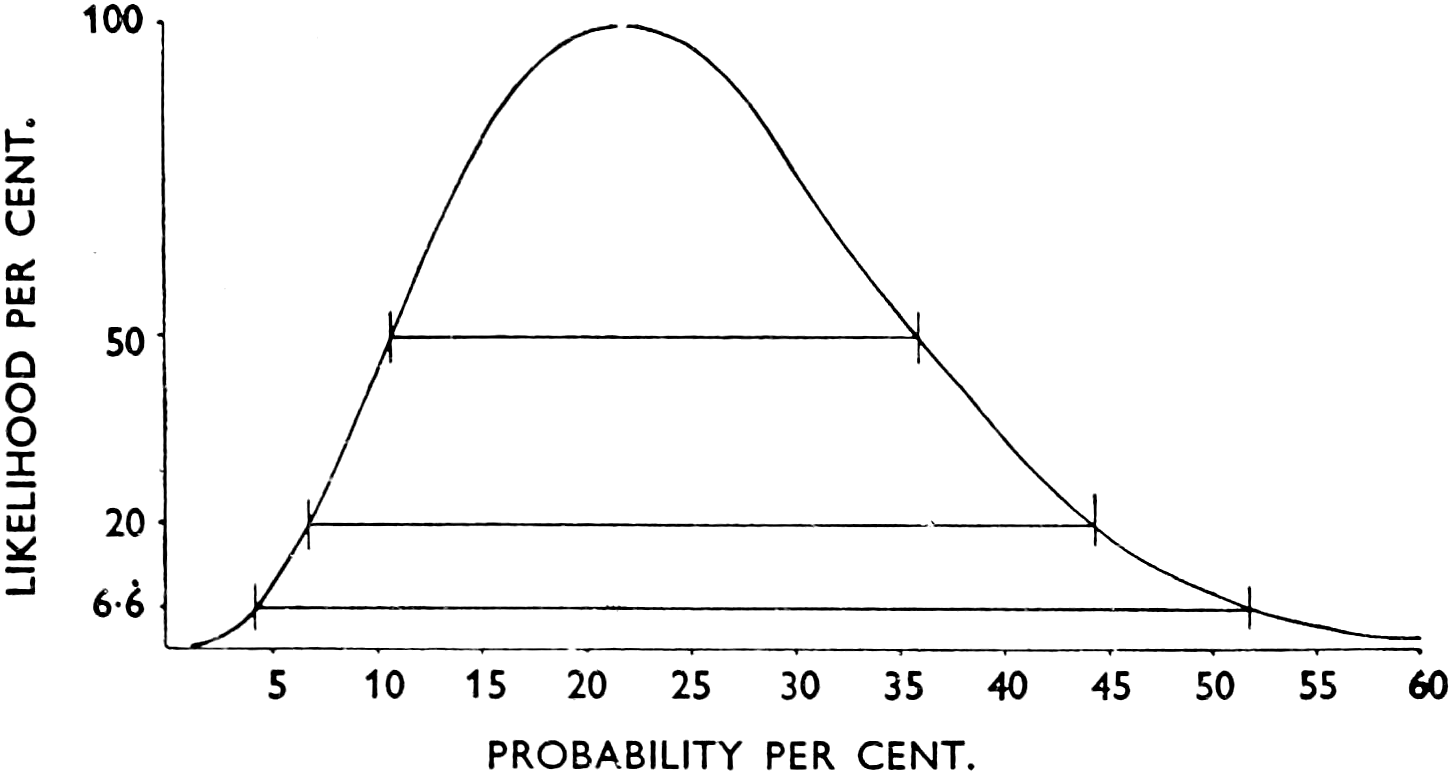
\includegraphics[width=0.95\textwidth]{figures/searches_fisher_likelihood_binomial.png}
\caption[
Intervals exceeding ratios from the maximum of a Binomial likelihood function,
reproduced from Fisher
]{%
Intervals exceeding ratios from the maximum of a Binomial likelihood function,
reproduced from Fisher~\cite{fisher1956statistical}.
Horizontal lines mark regions where the likelihood function exceeds
$1/2$, $1/5$, and $1/15$ of its maximum, respectively.
These lines could be tabulated to usefully summarize the profile of the
likelihood function.
}
\label{fig:searches_fisher_likelihood}
\end{figure}

\subsection{Fisher}
\label{sec:searches_fisher}
% likelihood
Fisher coined the term `likelihood'~\cite{
fisher1912fitting,
fisher1915frequency,
fisher1921probable,
fisher1922estimators
} in the usage that
we employ for the probability of observed data given varied
contexts,%
\footnote{%
Fisher used the term `likelihood' for the function exploring
contexts and `probability' for the distribution over
outcomes~\cite{fisher1925smrw}.
We choose the alternative word `prior' for his `probability' since the
likelihood is also a probability, just not a probability \emph{distribution}.
}
and deserves credit for popularizing its use in interpreting and communicating
data without the confounding influence of prior probabilities.
In his own words,%
\begin{quote}
\small
``%
We can know nothing of the probability of hypotheses or hypothetical
quantities.
On the other hand we may ascertain the likelihood of hypotheses
and hypothetical quantities by calculation from observations%
''~\cite{fisher1921probable},
\end{quote}
and furthermore we agree that in comparison to other prescriptions
(specifically confidence intervals, to be introduced in
Section~\ref{sec:searches_np}),
\begin{quote}
\small
``%
For all purposes, and more particularly for the \textit{communication} of the
relevant evidence supplied by a body of data, the values of the Mathematical
Likelihood are better fitted to analyse, summarize, and communicate
statistical evidence of types too weak to supply true probability statements%
''~\cite{fisher1956statistical}.
\end{quote}
For example, Figure~\ref{fig:searches_fisher_likelihood} displays a figure by
Fisher~\cite{fisher1956statistical} that illustrates how data can be usefully
reported by the likelihood's maximum and the regions in which it exceeds
certain ratios relative to that maximum.%
\footnote{%
We use such $L(\check{x})\pm\mathrm{ratio}$ visualizations for
$\pm1\sigma$ and $\pm2\sigma$ error bars on Poisson data in
Figure~7 of~\cite{lester2022hunting}.
When recommending error bar recipes, \atlas's statistics committee appears
to have not considered this option~\cite{cowan2011errorbars}.
% , although
% our statistics experts are surely familiar with Fisher's work.
}
That the likelihood contains all relevant information in the data is true by
definition in our formulation of Equation~\ref{eqn:searches_log_odds},
but non-Bayesian arguments find the same conclusion~\cite{
birnbaum1962foundations,
savage1962foundations
}.

Maximum likelihoods are often useful for interpreting and communicating data.
The location of a maximum likelihood can be a useful estimate for the
parameters being considered, and Fisher showed that maximum likelihood
estimates satisfy some desirable asymptotic
criteria~\cite{fisher1922estimators}.
These criteria do not include \emph{unbiasedness}, which states that the mean
value of an estimate --- over the distribution for alternative data --- should
equal its known true value~\cite{
sheynin1989aa,
Neyman1937Outline,
pdg2022ynf
}.
Defining bias as a difference from a mean fails to be coordinate-invariant,
so an unbiased estimate of the variance $\bar{\sigma}^2$ is a biased
estimate of the standard deviation $\bar{\sigma}$ --- the square of the mean
is not the mean of the squares~\cite{barlow2019svl}.
Fisher rejected the bias criterion for this
reason~\cite{jaynes2003probability}.
Other definitions absorb its
arbitrariness into an explicit loss function~\cite{lehmann2005testing}.
Requiring unbiasedness can actively harm results by preventing the use of
useful estimates,%
\footnote{%
Problem~1.14 of~\cite{lehmann2005testing} has a delightful example of
estimating an exponentiated a Poisson mean $\exp(\mu)$ from $n$ data
where the unique unbiased estimate is $(-1)^{n + 1}$.
Section~17.3 of~\cite{jaynes2003probability} shows similar nonsense for
unbiased estimates of $\mu^2$ and $\exp(-\mu)$.%
}
or by obfuscating those estimates with bias corrections.

Lingering uses of unbiasedness in high-energy physics~\cite{
pdg2022ynf,
Tullythesis,
lhcb2018563,
LHCb:2021trn,
LHCb:2015yax
}
are largely explained by the linguistic trickery of its name --- our
results should not be biased, and we like to report that to be true.
But we should proudly proclaim that our results are `biased' under this flawed
definition if that makes them better by any reasonable measure.

% likelihood quotes
In avoiding the pitfalls of reported posteriors, Fisher's use of likelihoods
remains innovative and practical.
However, the hard rejection of priors on hypotheses also prevents evidence
calculations, without which likelihoods alone can become confounded in many
parameters
(perhaps making those parameters seem feel more like `nuisances'
than useful levers).
To circumvent this, frequentist methods employ two key concepts:
test statistics, which can reduce the data to remove unwanted parameters,
and \pvalues, which divert the discourse
from what the alternative \emph{hypotheses are}
to what alternative \emph{data might have been}.

% test statistics
A statistic is a function of data, and a test statistic is just a statistic
that is used in statistical tests.
For \atlas\ collision data, event variables are statistics; when working with
data, one always uses statistics and is free to design them for their benefits
in context.
Just as we define event variables (like $\pt$) to remove nuisance
dependencies (on $\phi$ rotations or longitudinal boosts),
useful test statistics can also eliminate unwanted parameters.
The quintessential example is the $t$-statistic,
\begin{equation}
\label{eqn:searches_t_statistic}
t(d) = \frac{\bar{\mu}(d) - \mu}{\bar{\sigma}(d)/\sqrt{n}}
,
\end{equation}
which shifts the sample mean $\bar{\mu}(d)$ by a known true mean $\mu$, and
cancels any common scale factors with a scale-equivariant estimate of the
standard deviation $\bar{\sigma}(d)$~\cite{
student1908,
fisher1925t,
lehmann2011fisher
}.

One can usefully reduce observed data to just the test statistic
$\tilde{t} = t(d)$, and compare likelihoods on that observed $\tilde{t}$
to compare how well different hypotheses predict it.
Fisher, however, advocates a different use ---
rather than considering likelihoods here, he recommends
that researchers consider the ``probable error''~\cite{fisher1921probable},
which is a cumulative distribution function in the (negated) test statistic.
In modern jargon, a `probable error' with observed test statistic
$\tilde{t}$ and hypothesis $h$ is a \textbf{\pvalue}
\begin{align}
P(h)
&= \prob{t \geq \tilde{t}}{h}
\label{eqn:searches_pvalue}
\\
&= L(h) + \prob{t > \tilde{t}}{h}.
\label{eqn:searches_pvalue_likelihood}
\end{align}
The \pvalue\ $P(h)$ is the prior probability of data
\emph{greater or equal to} the observed data, if data are ordered by the value
of the test statistic.
Equation~\ref{eqn:searches_pvalue_likelihood} points out that the \pvalue\ is
just the likelihood plus some fluff from a tail of larger test statistics
(if the test statistic distribution is discrete).

Fisher illustrates the use of \pvalues\ in the second example
of~\cite{fisher1921probable}, which models some data with a parameter $r$ and
compares two hypotheses
$r=0.3$ and
$r=0.95$, finding \pvalues\
$P(r=0.3)=0.142$ and
$P(r=0.95)=0.00014$.
``Thus'', Fisher concludes, ``the value $0.95$\ldots\ is roughly $1000$ times
less likely than $0.30$''
(``when measured on the $r$ scale'').
By writing `likely', Fisher is carefully referencing their likelihoods,
not their probability.
But this factor of $1000$ is a \pvalue\ ratio, not a likelihood ratio,
so how can this make sense?
It could plausibly result from a tacit data reduction --- comparing
Equations~\ref{eqn:searches_pvalue} and~\ref{eqn:searches_likelihood}
shows that the \pvalue\ is a likelihood if the data statement is reduced from
$d_1: t =    \tilde{t}$ to
$d_2: t \geq \tilde{t}$.
And since this reduction is technically true --- $d_1$ implies $d_2$ --- the
likelihood ratio on $d_2$ is logically valid and not \emph{necessarily}
misleading if accurately reported.

However, $d_2: t \geq \tilde{t}$ is a logical statement (true for all test
statistics greater than or equal to the observed value) and not a randomly
occurring event; it therefore does not have a frequentist probability and so
is probably not what Fisher intended.
Much more importantly, the reduction to a one-sided inequality has no tangible
benefit --- it reduces the information content of the reported data without
reducing the associated costs of communicating or interpreting those data.
Both $d_1$ and $d_2$ are printed in the same number of characters, and
\pvalues\ can be painfully expensive to evaluate.
Furthermore, any result with a small test statistic is actively censored,
since if
\begin{equation}
\log \frac{L(h_1)}{L(h_2)}
\to
\log \frac{
L(h_1) + \prob{t > \tilde{t}}{h_1}
}
{
L(h_2) + \prob{t > \tilde{t}}{h_2}
}
\end{equation}
then large tail probabilities can only shrink the $\log$ likelihood ratio
towards zero.

Fisher's \pvalue\ ratio of $1000$ can therefore be a $\log$ likelihood
ratio of $+6.9$ in favour of $r=0.3$ over $r=0.95$, which is a notable
indication.
A likelihood ratio on the test statistic or data itself would however
encode more information and could provide a more precise answer.

\begin{figure}[tp]
\centering
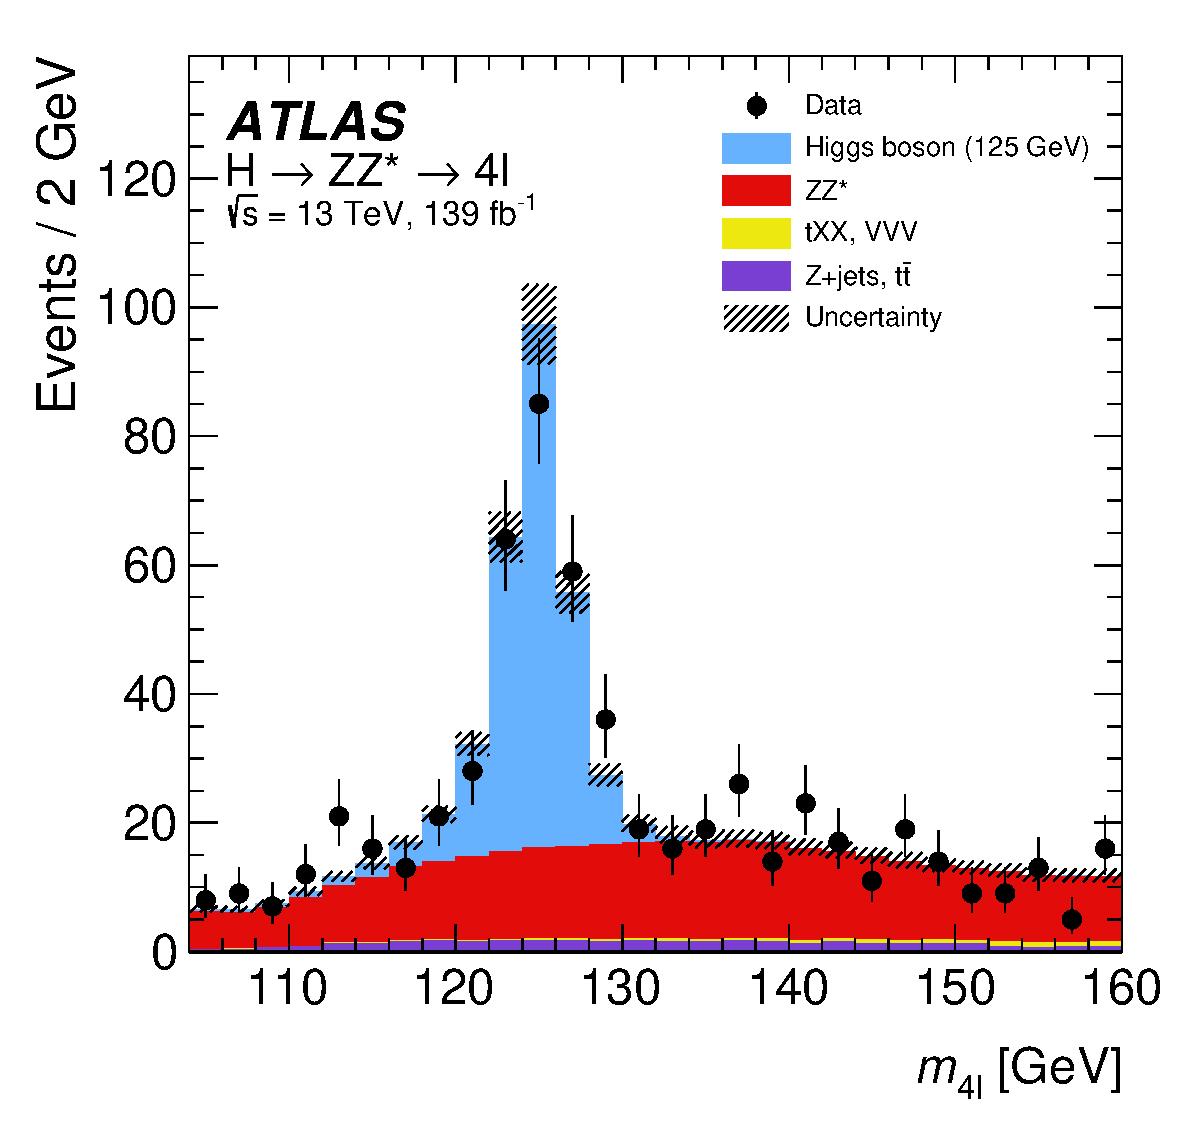
\includegraphics[width=0.6\textwidth]{figures/searches_atlas_higgs_4l_2207_00320.pdf}
\caption[
Signal and background distributions reproduced from the recent \atlas\
measurement of Higgs boson decays to $4\ell$
]{%
Signal and background distributions reproduced from the recent \atlas\
measurement of Higgs boson decays to $4\ell$~\cite{ATLAS:2022net}, with
observed data.
Because $m_{4\ell}$ would be a poor test statistic, this example illustrates
\pvalues' pathological dependency on tail selections and the usefulness of
likelihood ratios.
}
\label{fig:searches_atlas_higgs_4l}
\end{figure}

Fisher claims that the \pvalue\ indicates the ``significance'' of an
observation~\cite{fisher1925smrw}, with small or large values being
suspiciously significant, and that
``If $P$ is between $.1$ and $.9$ there is certainly no reason to suspect the
hypothesis tested.''~\cite{fisher1925smrw}
This may have been true for his intended applications, but it is not general;
as for other likelihoods, small values are only meaningful in comparison
against larger values from alternative hypotheses on the same data.

Consider for example the distributions of signal (Higgs boson) and background
(mostly $ZZ^*$) samples in Figure~\ref{fig:searches_atlas_higgs_4l}.
If an event is observed at $m_{4\ell} = 125\,\eV[G]$, is it signal or
background?
It is obviously a Higgs boson candidate, but $m_{4\ell}$ is around the middle
of both signal and background distributions, so with an $m_{4\ell}$ test
statistic $P(\textrm{Higgs boson}) \approx P(ZZ^*) \approx 0.5$ and neither
is `suspect'.
Local ratios between the two distributions clearly favour signal for this
event, however:
the \pvalues' failure is in their dependence on irrelevant tail areas,
which are a feature of the histogram and not the data.
This $ZZ^*$ density peaks for $ZZ$ above a
$2 m(Z) \approx 180\,\eV[G]$ kinematic edge,
and $Z \to 4\ell$ around $m_{4\ell} \approx m(Z)$~\cite{STDM-2017-09},
so expanding the histogram to show either of these tails would change nothing
local to our $m_{4\ell} = 125\,\eV[G]$ event, but would pathologically change
its \pvalues.

Better test statistics can soften this problem, and a key observation by
Neyman and Pearson is an optimality of likelihood ratio test statistics.


\subsection{Neyman-Pearson}
\label{sec:searches_np}
Suspecting an hypothesis when its \pvalue\ lands below (or above) a threshold
means that there is a prior probability $\alpha$ that any hypothesis will be
suspect after an experiment.
For example, in Fisher's suggestion of $P(h) \in 0.1\textrm{--}0.9$ being not
suspect, then $\alpha = 0.2$.%
\footnote{%
Matching $\alpha$ can be impossible in discrete distributions if
the tail probability masses do not add exactly to $\alpha$.
Neyman accommodates this by allowing inequalities with $\alpha$~\cite{
neyman1935Intervals
}.
Other approaches introduce ``extraneous randomization'' to
break up discrete distributions~\cite{tocher1950discontinuous}.
This problem of inexact `coverage' continues to cause controversy~\cite{
Read2002cls,
Feldman:1997qc,
cousins2008evaluation,
Cranmer2006Statistical
}.%
}
And that chance is independent of the hypothesis, its alternatives, and even
the nature of the experiment.

Obediently followed, these rules mean that the data and test statistic could be
anything at all and still incur suspicion for unrelated hypotheses with the
same prior probability ---
your wall clock reads greater than or equal to $48$ minutes past the hour?
If so, then the Standard Model is suspect.
Figure~\ref{fig:searches_significant} illustrates this peculiarity and the
associated difficulties with communicating \pvalue\ results.

\begin{figure}[tp]
\centering
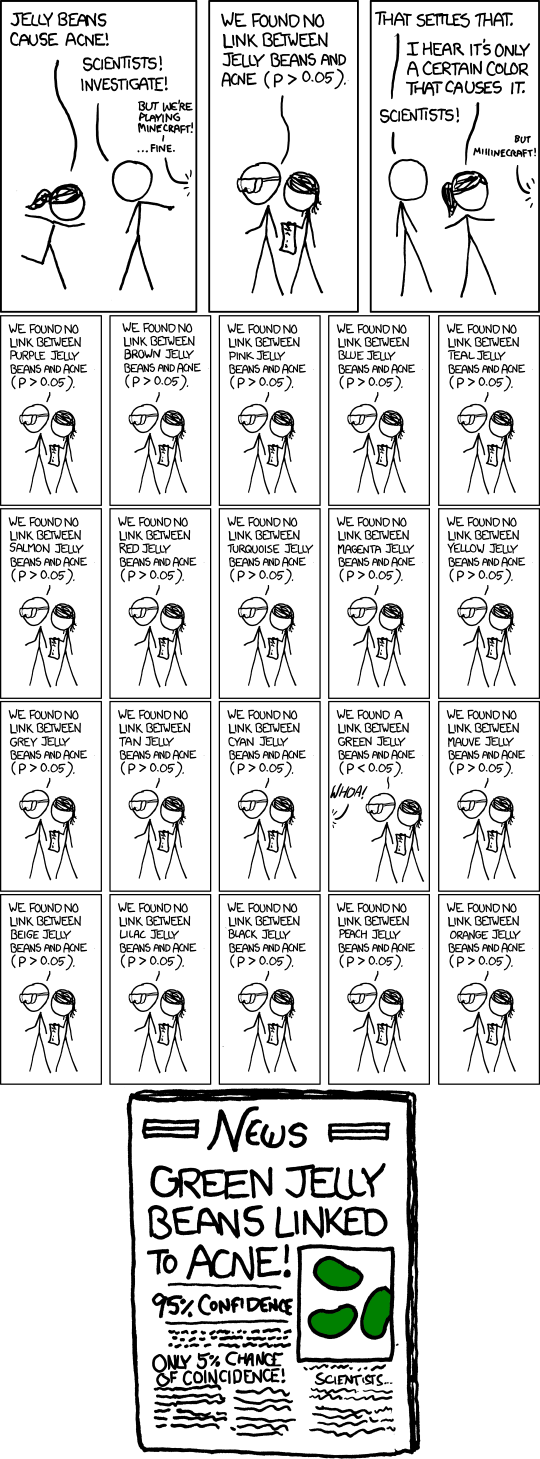
\includegraphics[width=0.46\textwidth]{figures/searches_significant_shrink.png}
\\
\begin{footnotesize}
`So, uh, we did the green study again and got no link. It was probably a{-}{-}'
\\
`RESEARCH CONFLICTED ON GREEN JELLY BEAN ACNE LINK; MORE~STUDY~RECOMMENDED!'
\end{footnotesize}
\caption[
``Significant'' from xkcd by Randall~Munroe
]{%
``Significant'' from xkcd by Randall~Munroe~\cite{xkcd2011significant}.
}
\label{fig:searches_significant}
\end{figure}

Neyman and Pearson formalized this `suspicion' into decision rules,
and considered what it is that makes one test statistic better than
another~\cite{neymanpearson1928max, neymanpearson1933lemma}.
Rather than a \pvalue\ arousing informal suspicion of an hypothesis, they use it
to decide on actions of `rejecting' or `accepting' an hypothesis.
From the same Bayesian arguments of Section~\ref{sec:searches_data_analysis},
Neyman and Pearson argued for the interest in likelihood ratios as promising
test statistics~\cite{neymanpearson1928max};
they also considered \emph{maximum} likelihood ratios
\begin{equation}
\label{eqn:searches_max_like_ratio}
\Lambda =
\frac{L(h_1)}{\mathrm{max}_i\,L(h_i)}
\end{equation}
to compare a specified hypothesis $h_1$ against a set of alternatives.

As descriptions of the likelihoods in play, maximum likelihood ratios can
usefully communicate relevant information from the data.
And as test statistics, they also win generality by avoiding context-specific
motivations, such as scale invariance for the $t$-statistic of
Equation~\ref{eqn:searches_t_statistic} --- any predictive models can have
likelihoods and maximum likelihood ratios.

``Without claiming that this method is necessarily the ``best'' to adopt,''
Neyman and Pearson suggest maximum likelihood ratios as
``one clearly defined method of discriminating between samples for which
Hypothesis A is more probable and those for which it is less probable''~\cite{
neymanpearson1933lemma}.
Lehmann appends ``(sic!)'' to this quote~\cite{lehmann2011fisher};
it appears to mistakenly conflate the likelihood for an hypothesis with its
probability, but Neyman and Pearson's association of likelihood ratios with
``more probable'' hypotheses may not be an error.
The authors understood the probability algebra of how large likelihood ratios
make hypotheses \emph{more probable} by scaling whatever (non-zero) prior
probabilities may be assigned.
Indeed, they later state that
\begin{quote}
``%
The statistician can balance the numerical verdict of likelihood against the
vaguer expectations derived from `a priori' considerations, and it must be left
to his judgment to at what point the evidence in favour of alternative
hypotheses becomes so convincing that Hypothesis A must be rejected.%
''~\cite{neymanpearson1933lemma}
\end{quote}
Elsewhere also, they consider an example with two hypotheses $\mathrm{A}_1$
and $\mathrm{A}_2$, and find a $\log$ likelihood ratio of
% the two corresponding densities at the sample point are
% ($\mathrm{A}_1$) $6.42 \times 10^{-20}$,
% ($\mathrm{A}_2$) $5.18 \times 10^{-4}$ and the ratio of the likelihood of
% Hypothesis $\mathrm{A}_1$ to that of $\mathrm{A}_2$ is $1.24 \times 10^{-16}$.
$-37$ and conclude that
``%
This ratio confirms the common-sense judgment that $\mathrm{A}_2$ is far more
plausible than $\mathrm{A}_1$%
''~\cite{neymanpearson1928max},
which again relates the likelihood ratio to how plausible an hypothesis is.

\begin{figure}[tp]
\centering
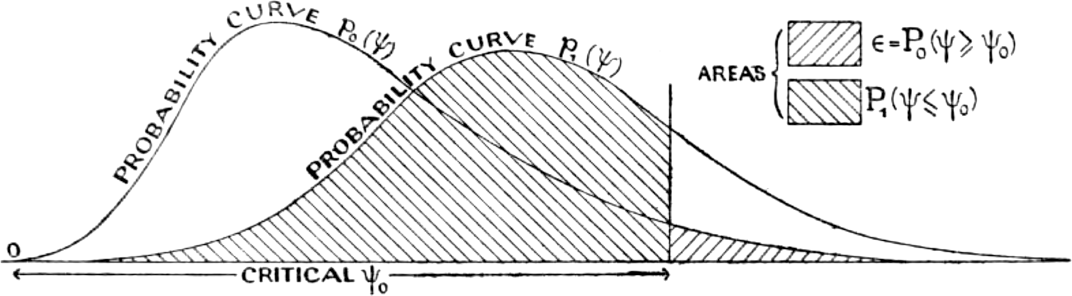
\includegraphics[width=0.95\textwidth]{figures/searches_np_curves_crop.png}
\caption[
Tail areas of prior probability distributions for data from two alternative
hypotheses, reproduced from Neyman and Pearson
]{%
Tail areas of prior probability distributions for data from two alternative
hypotheses, reproduced from Neyman and Pearson~\cite{neymanpearson1933lemma}.
}
\label{fig:searches_np_tails}
\end{figure}

The famous Neyman-Pearson lemma does not prove the usefulness of likelihood
ratios in probability algebra.
That was already known.
What it contributes is a relationship with one-sided inequalities ---
it states that likelihood ratios (not maximum likelihood ratios)
are optimal in a specific sense within their framework of decisions
based on \pvalues.
Precisely, at a fixed probability $\alpha$ of rejecting a true hypothesis,
the Neyman-Pearson lemma finds that a likelihood ratio test statistic maximizes
the probability $\alpha'$ of rejecting the alternative, false hypothesis that
lives in the denominator of the ratio; they illustrate this construction with
the diagram reproduced in Figure~\ref{fig:searches_np_tails}.

Only the likelihood ratio local to the observed data matters directly in the
probabilistic analysis, but this lemma is useful in the construction
of event variables of the kind we use in \atlas\ searches.
This is seen from the signal and background distributions of
Figures~\ref{fig:searches_sig_bkg_prior_likelihood}
and~\ref{fig:searches_atlas_higgs_4l}:
the event variable in Figure~\ref{fig:searches_sig_bkg_prior_likelihood} is
like a likelihood ratio in that any right-handed selection contains a good
signal purity relative to its background, but the signal bump in the
middle of the background distribution in
Figure~\ref{fig:searches_atlas_higgs_4l} would be better selected with a
window around the Higgs boson mass.
Re-ordering $m_{4\ell}$ by a likelihood ratio could turn the window
into an equivalent and simpler one-sided selection, and the Neyman-Pearson
lemma states that there is no ordering that further optimizes the selected
signal-to-background ratio.

Neyman and Pearson were also involved in the development of
`confidence intervals', which are ranges of parameters that are
accepted by a \pvalue\ decision rule~\cite{
clopper1934confidence,
neyman1935Intervals,
Neyman1937Outline
}.%
\footnote{%
Confidence intervals are usually introduced by endpoints containing constrained
probability mass, but this \pvalue\ form can always satisfy that through the
free choice of test statistic, and extends naturally beyond one dimension.%
}
A parameter corresponds to a hypothesis that assigns a prior distribution to
plausible data, and those data for which an obeisant researcher accepts the
hypothesis have probabilities that sum to $\gamma = 1 - \alpha$.
This $\gamma$ is known as the `confidence level'.
Such a rule selects a set of favoured data for each hypothesis, and the
confidence interval (when it can be constructed) contains hypotheses for which
the observed data are in that favoured set.

Confidence intervals are confusing.%
\footnote{%
Exemplifying such confusion,
the \atlas\ Glossary of Terms~\cite{atlas2022glossary} states that the
``Confidence Level (CL) is a statistical measure of the percentage of test
results that can be expected to be within a specified range.''
In fact, it is the percentage of ranges
(confidence intervals, which are test results)
that should cover a true value.%
}
It is easy to stumble into thinking that a confidence interval
`probably' contains the unknown parameter, but that gets it backwards.
For a known true parameter $x$, the various confidence intervals
$x_1\textrm{--}x_2$ from random repeated experiments should contain
$x$ with probability $\gamma$;
the interval makes a subtle statement about unknown alternative data for
known true parameters.
For given data, the confidence interval can even exclude all possible
parameters~\cite{
pratt1961testing,
Jaynes1976intervals
}.
Pratt succinctly explains the confidence interval by example:
\begin{quote}
\small
``%
A method yielding true statements with probability $.95$, when applied to your
experiment, yields the statement that your treatment effect is between $17$ and
$29$, but no conclusion is possible about how probable it is that your
treatment effect is between $17$ an $29$.%
''~\cite{pratt1961testing}.
\end{quote}
Neyman and Pearson never claimed otherwise; they did precise and rigorous
abstract mathematics, and confusion about their intervals arises
externally~\cite{jaynes2003probability}.

Confidence intervals are functions of the data, so they can inform vague
inferences if used as data for likelihood functions, just as we did to
interpret Fisher's \pvalue\ ratio as a likelihood ratio ---
an accurately constructed confidence interval $x_1\textrm{--}x_2$ has a
likelihood function:
\begin{equation}
L(x) =
\left\{
\begin{matrix}
\gamma & \textrm{if}~x \in x_1\textrm{--}x_2, \\
1 - \gamma & \textrm{otherwise.} \\
\end{matrix}
\right.
\end{equation}
And again, this reduction cannot add to the data.
It can only detract.
Fisher's recommendation to communicate the likelihood function itself
remains simpler and clearer.
In response to the idea that no conclusion can be drawn about the parameter,
Fisher also has strong words here:
\begin{quote}
\small
``%
There is something horrifying in the ideological movement represented by the
doctrine that reasoning, properly speaking, cannot be applied to empirical data
to lead to inferences valid in the real world.%
''~\cite{fisher1956statistical}
\end{quote}
Amen.

\begin{singlespacing}
\section{Post-frequentist practice}
\label{sec:searches_practice}
\begin{epigraphs}
\qitem{%
\ldots\ But this book, by its very excellence, its thoroughness, lucidity and
precision, intensifies my growing feeling that nevertheless the theory is
arbitrary, be it however ``objective,'' and the problems it solves, however
precisely it may solve them, are not even simplified theoretical counterparts
of the real problems to which it is applied.%
}%
{John~W.~Pratt,
\textit{Review: Testing Statistical Hypotheses},
1961~\cite{pratt1961testing}}
\end{epigraphs}
\end{singlespacing}
\noindent
Data analysis in modern high-energy physics does not exactly follow frequentist
ideology, but is a hands-on, practical, and evolving ecosystem that has adapted
to avoid some of the more glaring flaws when attacking real problems.
We have seen in Section~\ref{sec:searches_data_analysis} how likelihood ratios
can clearly express our scientific interest in how well competing models
predict data, and how those likelihoods can be manipulated in probability
algebra.
We have also seen in Section~\ref{sec:searches_frequentist} how 20th century
writers championed likelihoods not on the data themselves but on inequalities,
forming \pvalues\ and confidence intervals in reductions that throw away
information and obfuscate the results.
This section reviews how these objects are applied generally in conventional
analysis at the LHC, and specifically towards the \atlas\ search that this
thesis presents.

Misrepresentations of \pvalues\ (and other frequentist statistics) are
widespread and widely reported~\cite{
schervish1996p,
Cohen1994TheEI,
Amrhein2017TheEI,
goodman2008dirty,
greenland2016no,
Bernstein2016princess,
wagenmakers2007practical,
hauer2004harm,
wasserstein2016asa
}
in fields where they are not banned~\cite{
Trafimow2015ban,
woolston2015phychology,
chumra2019time,
shrout1997should,
hunter1997needed
}.
For example, the false presentation as a ``probability of compatibility'' with
a model~\cite{HIGG-2018-04} appears to be spreading as a good
meme~\cite{dawkins1989selfish} in high-energy physics~\cite{
roth2007fit,
HIGG-2017-09,
HIGG-2018-27,
HIGG-2018-51,
HIGG-2019-14,
EXOT-2016-36,
EXOT-2018-08,
EXOT-2019-15,
HION-2018-19,
chan2019search,
mastrandrea2019searches,
white2019search,
langford2021combination,
IceCube2013search,
IceCube2014searches,
gerasimov2021new
},
and is plausibly explained by mutations from vaguely accurate statements like
``compatible with the SM prediction with a p-value of $0.10\%$''~\cite{
lhcb2021test
}
to precisely inaccurate statements like
``a probability of around $0.1\%$ that the data is compatible with the
Standard Model predictions''~\cite{cern2021test}.

There also exists a notion that a small \pvalue\ means that the data
represent a rare fluctuation~\cite{murray1997use, atlas2022glossary}.%
\footnote{%
The \atlas\ Glossary of Terms~\cite{atlas2022glossary} falsely states that
``The \textbf{p-value} is the probability (ranging from $0$ to $1$) that the
results observed could have occurred by chance, if the tested theory has no
impact on the study.''%
}
All \pvalues\ are rare.
By construction, they are uniformly distributed between $0$ and $1$, so the
probability that $P(h) < \varepsilon$ equals the probability that
$0.4 \leq P(h) < 0.4 + \varepsilon$ or that it lands in any
$\varepsilon$-sized set,
if the data are sampled under $h$.
What matters to our interpretation is whether an alternative hypothesis
makes the observed result \emph{more probable}.

\subsection{\texorpdfstring{$\cls$}{CLs}}
\label{sec:searches_cls}
Such misrepresentations of our results reinforces the need for clearer
replacements, which $\log$ likelihood ratios can provide.
Standard practice at the LHC contains the beginnings of such
replacements under the name $\cls$~\cite{
read2000modified,
Read2002cls,
junk1999confidence,
read1997optimal,
bock1998lower,
etde1998prospects,
lep2000searches,
lep2003search,
Murray2010heretic,
cern2011procedure,
pdg2022ynf
},
which is used for setting upper limits on disfavoured signal yields $s$
above background yields $b$:
\begin{equation}
\label{eqn:searches_cls}
\cls
=
\frac{P(s + b)}{P(b)}
=
\frac{
\prob{t \geq \tilde{t}}{s + b}
}{
\prob{t \geq \tilde{t}}{b}\hfill
}
,
\end{equation}
in which the individual \pvalues\ are named
$\clb = P(b)$ and
$\clsb = P(s + b)$.%
\footnote{%
Despite their $\mathrm{CL}$ labels, $\cls$, $\clsb$, and $\clb$ are not
Confidence Levels ---
a confidence level $\gamma$ is a threshold used to assign limits by solving
for $x$ such that $\gamma = 1 - P(x)$~\cite{pdg1996}.
In particle physics, \pvalues\ have sometimes been labelled $\mathrm{CL}$ since
at least 1984~\cite{pdg1984}, although textbooks from the '70s (which are cited
by~\cite{pdg1984}) do distinguish between the two~\cite{
eadie1971statistical,
frodesen1979probability
}.%
}%
\footnote{%
Some literature defines $\clb = 1 - p_b$~\cite{
Cowan:2010js,
pdg2022ynf
},
in which $p_b$ might not be a \pvalue\ if it excludes equality with the
observed test statistic~\cite{cern2011procedure}.
}

As discussed in Section~\ref{sec:searches_fisher}, \pvalues\ are likelihoods
on obfuscated data, so (with some caution) $\cls$ can be interpreted as a
likelihood ratio.%
\footnote{%
Likelihood ratios are useful if both their numerator and denominator use the
same data, so $\clsb$ and $\clb$ should use the same test statistic.
Identical test statistics are used for all results in this thesis, but
differing test statistics have been allowed elsewhere~\cite{bock1998lower}.
}%
At a given confidence level $\gamma$ (typically $95\%$), limits are set to
values of $s$ for which $\cls = 1 - \gamma$.

Early variants of $\cls$ derived it from an identity with posterior tail
probabilities in Poisson and Gaussian special cases~\cite{
Helene1983upper,
pdg1988,
read2000modified,
pdg2022ynf
}
with a contrived frequentist interpretation~\cite{zech1988cls}.
For use in general cases, it is more recently described as a
``modified frequentist'',
``approximate confidence in the signal-only hypothesis''~\cite{
read2000modified,
Read2002cls
}.
High-profile usage in combined Higgs boson searches at LEP~\cite{
read1997optimal,
bock1998lower,
etde1998prospects,
junk1999confidence,
lep2000searches,
lep2003search
}
appears to have propelled $\cls$ to prominence;
these early applications used data deficits to exclude their
background-plus-signal models, sometimes with the test statistic $t(n) = -n$,
and disliked how deficits led to small \pvalues\ for the background-only model,
with which they might have confusingly set negative limits on the Higgs boson
signal cross-section.
Such \pvalues\ are illustrated in Figure~\ref{fig:searches_sb_n} (left)
for small data counts;
in contrast, $\cls$ can only favour the background-only model, due to its
negative values that are shown on the right of the same figure.

\begin{figure}[tp]
\centering
\begin{subfigure}{\textwidth}
\centering
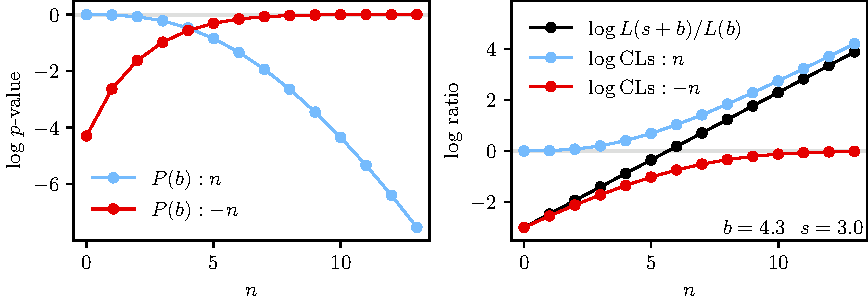
\includegraphics[width=\textwidth]{figures/searches_cls_plots_with_pvals_n.pdf}
\end{subfigure}
\caption[
A Poisson model in the natural order
]{%
A Poisson model in the natural order of $t(n) = \pm n$
test statistics, $b = 4.3$ and $s = 3.0$.
(left) $\log$ \pvalues,
and (right) $\log$ likelihood ratios and $\log$ $\cls$ for
background and signal-plus-background models.
The $n$ test statistic is Neyman-Pearson optimal because it is monotonically
(linearly) related to the likelihood ratio.
Each $\cls$ is a \pvalue\ ratio with the stated test statistic.
By reducing the observed data to an inequality, the \pvalue\ selectively
censors its information.
}
\label{fig:searches_sb_n}
\end{figure}

Despite my statement in Section~\ref{sec:searches_fisher} that \pvalue\
ratios are not ``not \emph{necessarily} misleading'',
Figure~\ref{fig:searches_sb_n} shows a bias from the fact that
no data can give a $\cls$ that favours the signal model;
$\log\cls$ is non-positive with the $-n$ test statistic, and non-negative
for the reverse ordering $t(n) = n$.
The $\log$ likelihood ratio on the actual data does not feature this bias:
it favours background-only for deficits and background-plus-signal for
excesses.
The $\log$ likelihood ratio is linear in $n$ for these Poisson models,
\begin{equation}
\log \frac{L(s + b)}{L(b)}
= n\log\frac{s + b}{b} - s
,
\end{equation}
so both $n$ and $-n$ can be optimal in the Neyman-Pearson sense.

By using $\cls$ with a Neyman-Pearson optimal test statistic, we have therefore
constructed an analysis that can only ever favour one hypothesis:
we have built a propaganda machine, which only ever speaks truth,
but which censors any information that supports alternative ideas.
Reducing data to inequalities $t \geq \tilde{t}$ implements the censorship,
and the likelihood-ratio ordering guarantees the one-sided inferences
that appear in Figure~\ref{fig:searches_sb_n} (right) as one-sided
$\log\cls$ values.

\begin{figure}[tp]
\centering
\begin{subfigure}{\textwidth}
\centering
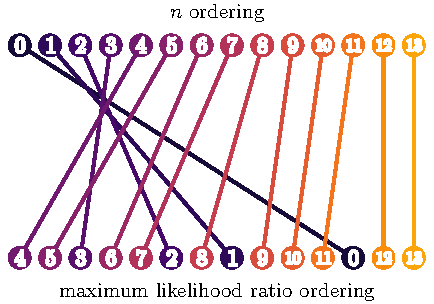
\includegraphics[width=0.6\textwidth]{figures/searches_cls_plots_with_pvals_order.pdf}
\caption{%
Ordering the data by a maximum likelihood ratio test statistic with $b=4.3$.
Data on the top are ordered with $n$ increasing from left to right,
and on the bottom those same data are reordered to have increasing values of
test statistic $t(n) = -\Lambda(n)$.
}
\end{subfigure}
\\[.5em]
\begin{subfigure}{\textwidth}
\centering
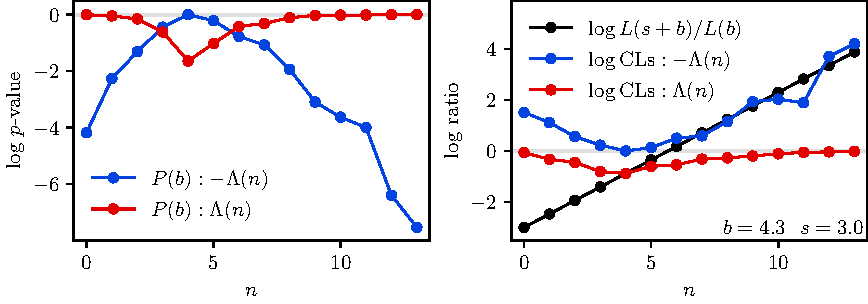
\includegraphics[width=\textwidth]{figures/searches_cls_plots_with_pvals_t.pdf}
\caption{%
(left) $\log$ \pvalues\ for Poisson data,
and (right) $\log$ likelihood ratios and $\log$ $\cls$ for
background and signal-plus-background models.%
}
\end{subfigure}
\caption[
Analysis of a minimal Poisson model with maximum likelihood ratio
test statistics
]{%
Analysis of a minimal Poisson model with maximum likelihood ratio
test statistics $t(n) = \pm \Lambda(n)$,
where $\Lambda(n) = L(b)/\mathrm{max}_x\,L(x)$; $b = 4.3$ and $s = 3.0$.
This test statistic jumbles the data into an order that makes $n=11$ appear to
be weaker support for the signal than $n=9$.
Each $\cls$ is a \pvalue\ ratio with the stated test statistic.
By reducing the observed data to an inequality, the \pvalue\ selectively
censors its information.
}
\label{fig:searches_sb_t}
\end{figure}

How can one escape this trap?
Likelihood ratios on the actual data escape immediately by by-passing the
censor, but even inequalities need not be biased if models can ask
questions of the data and be given honest answers.
For example, if asking whether the data exceed a predetermined threshold
of  $5$ events, then the truth or falsehood of `$n \leq 5$'
can favour either side.

With multiple Poisson bins, the $n$ test statistic is no longer
sufficient.
In such general cases, maximum likelihood ratio test statistics,
such as $\Lambda$ of Equation~\ref{eqn:searches_max_like_ratio}, are often
useful.
With a single bin, $\Lambda$ shuffles the ordering of
data and leads to some odd features in the results, which are displayed in
Figure~\ref{fig:searches_sb_t}.
In particular, the choice $t(n) = -\Lambda(n)$ pushes any data that are far
from the background expectation into its tails, so can disfavour the background
model for small $n$.
Probability masses from small data also interrupt its behaviour for excesses,
and lead to jagged changes, notably that $\log\cls$ reduces as the data
increase from $9$ to $11$.
Counter to intuition and logic, this prescription can report decreased favour
for the signal model when increasing the excess in data.

Rather than $\Lambda$ itself, various modified maximum likelihood ratio test
statistics enjoy standard usage at the LHC~\cite{cern2011procedure};
these are variably defined as piecewise functions of the fitted signal
parameter, and can include likelihoods from the signal-plus-background
model with constrained maximizations, which aim to reduce the impact of
unphysical results such as negative Poisson expectations~\cite{
Feldman:1997qc,
Cowan:2010js
},
and can improve (in a context-dependent sense) the resulting ordering.

Modified maximum likelihood ratios also benefit from known approximations to
their sampling distributions in asymptotic (Gaussian) limits,
which can assign their \pvalues\ through well-behaved analytic
expressions~\cite{
Cowan:2010js,
wilks1938large,
wald1943tests
}.%
\footnote{%
Remarkably, the asymptotic limits employed by~\cite{Cowan:2010js} to
approximate \pvalues\ derive from a theorem of the same Abraham~Wald who later
proved the redundancy of \pvalue\ decision rules~\cite{wald1947bayes}.%
}
Without such formulae, the remaining practical approach to estimating
\pvalues\ is to generate Monte Carlo simulations of alternative data.
However, such simulations can be computationally expensive, and ill-defined for
``likelihood'' models that blur the distinction between actual data and
auxiliary constraints.


\subsection{Likelihood modelling}
To represent the Standard Model and alternatives, LHC data analyses use
parametric models to describe the models' Poisson expectations of
collision events and how those expectations change in response to their
parameters.
Parameters often correspond to interpretable, physical quantities and when
those parameters are known only with some uncertainty, the models help to
propagate uncertainty into variations of their outputs.

Uncertainties on imperfectly-known yet non-random parameters, however,
conflict with the frequentist denial of prior probabilities.
To avoid this, all modelling is officially framed as not predicting parameters,
but instead constraining them with likelihood functions that use
either real control data or fictional auxiliary data.

This transformation of priors to auxiliary likelihoods is generally possible
--- in a prior density $f(x)\,\mathrm{d}x$, the function $f(x)$ is a likelihood
(strictly, a Radon-Nikodym derivative~\cite{billingsley2008probability})
that constrains the (possibly non-normalized or `improper') prior measure that
is uniform in $x$~\cite{Cowan:2010js}.
But as discussed in Section~\ref{sec:searches_probability_applied}, the shape
of $f(x)$ is entirely determined by the coordinate, and is therefore a free
choice made by the analyst.
By assigning a form to the auxiliary likelihood, therefore, one is really
choosing a \emph{regularizer} that should be intended to induce preferable
behaviours in the parametric model and its `maximum likelihood' statistics.

These regularized models with constraints from fictitious auxiliary data
are usually often ``likelihood'' models~\cite{
cranmer2012histfactory,
baak2015histfitter,
Besjes_2015,
heinrich2021pyhf
}.
To distinguish them from real likelihood functions on actual data, this
thesis uses the alternative spelling \textbf{\heplikelihood}.

Many of our uncertainties do not correspond to predictions of auxiliary data:
examples include
scale variations,
theoretical cross-section uncertainties,
non-closure uncertainties (which cover differences between estimates),
simulated sample comparisons,
statistical errors on weighted simulations,
extrapolation uncertainties,
and
all uncertainties on supersymmetric signal yields
(for which we have yet no data).
We describe these uncertainties by heuristically
combining theoretical modelling, physical intuition, and convention,
and not only by measuring random data.
Believing that they are also likelihoods on auxiliary data is
doublethink~\cite{orwell1949nnineteen}.

Despite their troublesome nomenclature, \heplikelihood\ models are extremely
useful and effective for describing the predictions of our hypotheses and
extracting interpretable results.
A general \heplikelihood\ model is a function $H(x)$ that takes input
parameters $x$ and outputs two things:
expected yields $y(x)$ to predict Poisson data,
and an objective value $E$ to be minimized (in a `fit') to choose a best
prediction.
That is,
\begin{equation}
H(x) = [\,y(x), \,E(x)\,]
.
\end{equation}
The minimization objective $E$ is the summed negative $\log$ \heplikelihood\
for all actual and auxiliary data.
We choose the letter $E$ for \textbf{energy}, to highlight the analogy with
statistical physics and the Boltzmann factor
$f(x) \propto e^{-E(x)/(k_B T)}$,
with which a thermodynamic system collapses to its minimum energy at cold
temperatures~\cite{
skilling2017david,
lecun-06,
pmlr-v2-ranzato07a
}.
At unit temperature, this can induce a probability distribution
relative to an appropriate measure~\cite{
cranmer2012histfactory,
skilling2017david
},
but in my experience with \heplikelihood\ models such distributions often
coincide with neither intuition nor the best fit value.%
\footnote{%
One can reproduce this experience by sampling a public \pyhf\ \heplikelihood\
model
(for example, try SR-HM(disc.) of $1\ell bb$~\cite{SUSY-2019-08,hepdata.90607})
with standard Markov-Chain Monte Carlo algorithms.
I recommend first estimating the covariance by expanding about the maximum
\heplikelihood, and linearly transforming your coordinates to whiten that
covariance to the identity matrix.
Then, algorithms provided by
TensorFlow Probability~\cite{tensorflow2015-whitepaper}
(the Metropolis-Adjusted Langevin Algorithm~\cite{mala1998, XIFARA201414}
is a good start)
can sample quite efficiently with tensor evaluation through
\pyhf~\cite{heinrich2021pyhf}.
Histograms of samples for the signal strength in the discovery fits
can differ substantially from profile-\heplikelihood\ curves.
}

Error bars on the yields can be assigned by exploring around that best fit.
In the Gaussian approximation, the inverse (Hessian) matrix of second
derivatives gives a covariance matrix in the parameters from which linear
projections can estimate the variance of any output.
The second derivatives of exactly Gaussian forms are independent of the
parameter point, but since we do not have exactly Gaussian models we evaluate
these derivatives about the best fit point, either analytically or with finite
difference approximations~\cite{cranmer2021building}.
Other practical approaches explore parameter ranges in which the minimum energy
exceeds thresholds.

All results presented in this thesis use
\histfactory~\cite{cranmer2012histfactory} \heplikelihood\ models that are
constructed and analysed with
\histfitter~\cite{Besjes_2015,baak2015histfitter}
and \pyhf~\cite{heinrich2021pyhf}.
\histfactory\ models are specialized for working with discrete histogram bins.
They constrain parameters with either Gaussian or Poisson%
\footnote{%
Poisson likelihoods in these software packages typically use a continuous
interpolation with $n! \to \Gamma(n + 1)$.%
}
likelihood
functions, and assign expected yields through a variety of
non-linear functions of the parameters.
Each parameter's effect is generally described by
\emph{central}, \emph{high}, and \emph{low}
(corresponding to the best and $\pm1\sigma$)
values of modifications to bin yields.%
\footnote{%
Because extrapolations from the variations are non-linear, the exact forms of
the constraints do not directly matter.
Numerical optimizers prefer Gaussian forms for their $\log$ quadratic shape, which is
easily minimized in the common case that the parameter has no observable
effect.%
}

Along with each \heplikelihood\ constraint, \histfactory\ also assigns a
sampling distribution for alternative values of its (auxiliary) data.
To approximate \pvalues\ without the asymptotic approximations,
these distributions are used in a standard procedure for simulating
alternative ``pseudo-data (toys)''~\cite{cern2011procedure}.
This procedure works as follows:
\begin{enumerate}
\item minimize $E(x)$ to find the best-fit parameters $\check{x}$, then
\item at fixed $\check{x}$, sample alternative Poisson (actual) data with rates
$y(\check{x})$ and alternative auxiliary (fictitious) data from their assigned
distributions, then
\item evaluate the test statistic for each simulated `toy'
sample~\cite{cern2011procedure}.
\end{enumerate}
Each \pvalue\ is estimated as the fraction of sampled toys with test statistics
greater than or equal to the observed test statistic.
Because this first item fits to the observed data, the sampled test statistic
distribution depends on the observed data $d$ ---
this is problematic because it means that the approximated \pvalue\ is not
$\prob{t \geq t(d)}{h}$, but depends on the data like
$\prob{t \geq t(d)}{f(d, h)}$.
And since the \pvalue\ is a censored likelihood value%
\footnote{%
As argued in Section~\ref{sec:searches_cls}.%
}, this is an error of early
unblinding, or, in machine-learning-speak, training on the test set.
It can make little difference when the yields are insensitive to the observed
data, but we shall see an example (of DR-Low) in
Section~\ref{sec:2ljets_results} where they are sensitive, and where
this makes a deficit in data appear much less significant than it  otherwise
would.
Sampling alternative data from fixed $y(\check{x})$ is also suspicious because
we are in fact uncertain of the expected yields,
as demonstrated by the error bars we draw on them.

Nonetheless, this procedure often simulates reasonable-looking test statistic
distributions, does not rely on asymptotic approximations, and purportedly
has ``good coverage properties''~\cite{
cern2011procedure,
Cranmer2006Statistical
}.
Toy simulation is an approximation, and in given circumstances may be better or
worse than the asymptotic approximations.
% Pick your poison.


\subsection{\atlas\ SUSY searches}
\label{sec:searches_searches}
Searches for new effects from supersymmetric models in \atlas\ face the problem
that their signals often appear in obscure, extreme, or otherwise less-studied
corners of the data.
In \atlas\ SUSY searches, our modelling of the  Standard Model is therefore
treated with substantial suspicion, and we tune that modelling to better
describe the backgrounds local to our data of interest before finalizing a
search.
Tuning and analysis are performed in a conventional and sensible procedure,
but their pieces have esoteric names that we define here.

Our searches see data only through discrete histogram bins named `regions',
which are defined by logical selections in event variables.
To communicate their intended uses, we further categorize these bins into
`control', `validation', and `signal' regions;
Figure~\ref{fig:searches_histfitter_regions} illustrates the uses of these
three region types.

\begin{figure}[tp]
\centering
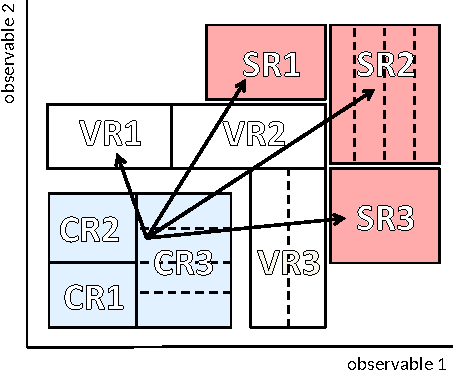
\includegraphics[width=0.6\textwidth]{figures/searches_histfitter_regions.pdf}
\caption[
Control, validation, and signal regions
]{%
Control, validation, and signal regions and the extrapolation between them.
Both observables are event variables in which models should change
smoothly to justify the extrapolations that are indicated by arrows.
Dashed lines illustrate that each region may be subdivided into
disjoint (orthogonal) smaller bins.
Adapted from \histfitter~\cite{baak2015histfitter}.
}
\label{fig:searches_histfitter_regions}
\end{figure}

\paragraph{Control regions (CRs).}
Control regions select large numbers of data to constrain global normalization
factors that scale Standard Model backgrounds;
these normalization factors control the total cross-sections of
background samples while preserving their relatives shapes between regions.
Disregarding theoretical Standard Model cross-sections is justified, since
the control region constraints are, by design, more precise than any previous
estimate local to our regions.

\paragraph{Validation regions (VRs).}
To represent the Standard Model, control regions must be insensitive to
non-standard signals.
Before applying their normalization factors to regions that are sensitive
to signal hypotheses, data in validation regions are first used to test the
quality of extrapolation.
Each model is adjusted until validation region data are well predicted ---
either by changing region definitions or restructuring the \heplikelihood\
model, perhaps with extrapolation uncertainties or extra normalization
factors.
No Poisson likelihoods for validation region data are included in the
\heplikelihood\ models, but their data are important and indirectly used to
update the model in this manner.

\paragraph{Signal regions (SRs).}
Consuming information from control and validation regions to refine the
predictions of our background-only model is scientific learning, and can be
reconciled with machine learning practice as fitting a model with training
(CR) and validation (VR) data.
Final testing is done by predicting of data in the signal regions, in which
signal models could have significant effects.
Some signal regions are labelled as \textbf{discovery regions} (\textbf{DRs})
to indicate their use in special `discovery' fits.

Various fits are useful to extract different results from search regions.
We briefly describe the three classes of fit here, and shall see examples
of their results in Chapter~\ref{chapter:2ljets}.

\paragraph{Background-only fits.}
With no signal contribution present, the background-only model is fitted
to the control regions to make predictions in the signal regions.
These background-only fits usefully validate that the \heplikelihood\ model
works as intended: that its normalization factors are not too far from the
Standard Model, that its tuned extrapolation to validation regions works,
and that other parameters are behaving as intended.

After fitting the background-only model to observed signal region data,
it can be useful to check whether its parameters have been `pulled' away from
their central values into regimes where their approximated extrapolations may
be invalid.
Post-fit expectations in signal regions are also available with error bars;
because these depend on the data, they are posterior results and not directly
useful to judge the background-only model.
Instead, they are an updated prediction of the expected yields from an
hypothetical future repeat of the experiment.

Searches for new signals require some concept of how their signals differ
from the backgrounds;
\atlas\ SUSY searches consider two such concepts with two flavours:
exclusion fits, and discovery fits.

\paragraph{Exclusion fits.}
Model-dependent `exclusion' fits add simulated yields from precisely
defined models to the \heplikelihood\ model.
These fits can use multiple signal regions simultaneously, and couple the
effect of parametrized modifications to the signals and backgrounds between
the bins of those regions.

From exclusion fits, we extract statistical results with the $\cls$ method to
mark individual models as excluded and set limits on their production
cross-sections.
For presentation on paper, articles consider two-dimensional planes of model
parameters and present contiguous `exclusion contours' within which all models
are marked as excluded.

\paragraph{Discovery fits.}
Model-dependence sacrifices some generality.
Model-independent `discovery' fits are therefore performed to extract results
that could be interpretable for any hypothesized model.
These fits include the control regions and only one signal region, a
discovery region, in which a flat signal yield is considered.
The $\cls$ method is again used to set limits on that signal yield,
and a `discovery' \pvalue\ is also computed with the intention to quantify
the significance of a data excess were one observed.

Despite the likely superiority of $t(n) = n$ test statistics for these
single-bin data, maximum likelihood ratio test statistics are used as standard,
and may explain quirks in the discovery region results that we shall see in the
results of Chapter~\ref{chapter:2ljets}.

% this comment activates enlarged spacing for the final paragraph lol
